\documentclass[conference]{IEEEtran}

\usepackage{amsmath,bm}
\usepackage{graphicx}
\def\MLine#1{\par\hspace*{-\leftmargin}\parbox{\textwidth}{\[#1\]}}
\graphicspath{ {./Images/} }

%%%%%%%%%%%%%%%%%%%%%%%%%%%%%%%%%%%%%%%%%%%%%%%%%%%%%%%%%%%%%%%%%%%%%%%%%%%%%%%%%%%%%%%%%%%%%%%%%%%%%%%%%%
\begin{document}
%%%%%%%%%%%%%%%%%%%%%%%%%%%%%%%%%%%%%%%%%%%%%%%%%%%%%%%%%%%%%%%%%%%%%%%%%%%%%%%%%%%%%%%%%%%%%%%%%%%%%%%%%%
\title{1: Introduction}
\author{Xin Wang}
%%%%%%%%%%%%%%%%%%%%%%%%%%%%%%%%%%%%%%%%%%%%%%%%%%%%%%%%%%%%%%%%%%%%%%%%%%%%%%%%%%%%%%%%%%%%%%%%%%%%%%%%%%
\maketitle
%%%%%%%%%%%%%%%%%%%%%%%%%%%%%%%%%%%%%%%%%%%%%%%%%%%%%%%%%%%%%%%%%%%%%%%%%%%%%%%%%%%%%%%%%%%%%%%%%%%%%%%%%%
\section{What is a signal}
%%%%%%%%%%%%%%%%%%%%%%%%%%%%%%%%%%%%%%%%%%%%%%%%%%%%%%%%%%%%%%%%%%%%%%%%%%%%%%%%%%%%%%%%%%%%%%%%%%%%%%%%%%
\begin{itemize}
  \item A function of one or more variables representing data
  \item Represented by a physical aspects e.g. voltage
  \item Measured by observing physical aspects
\end{itemize}

%%%%%%%%%%%%%%%%%%%%%%%%%%%%%%%%%%%%%%%%%%%%%%%%%%%%%%%%%%%%%%%%%%%%%%%%%%%%%%%%%%%%%%%%%%%%%%%%%%%%%%%%%%
\section{Types of signals}
%%%%%%%%%%%%%%%%%%%%%%%%%%%%%%%%%%%%%%%%%%%%%%%%%%%%%%%%%%%%%%%%%%%%%%%%%%%%%%%%%%%%%%%%%%%%%%%%%%%%%%%%%%
\subsection{Continuous-time and discrete-time}

\begin{itemize}
  \item Continuous: 
  \begin{itemize}
    \item Signal defined for all time $t$
    \item E.g. sound
  \end{itemize}
  \item Discrete: 
  \begin{itemize}
    \item Signal defined only at discrete instants of time $nT_s$
    \item E.g. Digital music
  \end{itemize}
\end{itemize}

%%%%%%%%%%%%%%%%%%%%%%%%%%%%%%%%%%%%%%%%%%%%%%%%%%%%%%%%%%%%%%%%%%%%%%%%%%%%%%%%%%%%%%%%%%%%%%%%%%%%%%%%%%
\subsection{Even and odd}

\begin{itemize}
  \item All signals composed of even and odd components
  $$
    x(t) = x_e(t) + x_o(t)
  $$

  \item Even:
  $$
    x_e(t) = \frac{1}{2}[x(t) + x(-t)]
  $$
  \begin{itemize}
    \item Positive and negative are the same
    $$
      x_e(t) = x_e(-t)
    $$
  \end{itemize}

  \item Odd:
  $$
    x_o(t) = \frac{1}{2}[x(t) - x(-t)]
  $$
  \begin{itemize}
    \item Positive and negative are different
    $$
      x_o(t) = -x_o(-t)
    $$
  \end{itemize}
\end{itemize}

%%%%%%%%%%%%%%%%%%%%%%%%%%%%%%%%%%%%%%%%%%%%%%%%%%%%%%%%%%%%%%%%%%%%%%%%%%%%%%%%%%%%%%%%%%%%%%%%%%%%%%%%%%
\subsection{Periodic and non-periodic}

\begin{itemize}
  \item Continuous-time periodic $T_0$ signal:
  $$
    x(t) = x(t + T_0) \; \forall t
  $$
  where $T_0$ is the \textbf{fundamental period}

  \item Discrete-time periodic $N_0$ signal:
  $$
    x[n] = x[n + N_0]
  $$
  with \textbf{fundamental angular frequency} $\Omega_0 = \frac{2\pi}{N_0}$
  
\end{itemize}

%%%%%%%%%%%%%%%%%%%%%%%%%%%%%%%%%%%%%%%%%%%%%%%%%%%%%%%%%%%%%%%%%%%%%%%%%%%%%%%%%%%%%%%%%%%%%%%%%%%%%%%%%%
\subsection{Deterministic and Random signals}

\begin{itemize}
  \item \textbf{Deterministic signal}: Specified function of time i.e. no uncertainty about signal
  value at any observed instant of time 

  \item \textbf{Random process}: Describes group of random signals 
  \item \textbf{Random signal}: Cannot be determined before occurring
  \begin{itemize}
    \item Different waveform and occurring probabilities
    \item A particular occurrence of a random process 
  \end{itemize}
\end{itemize}

\pagebreak
%%%%%%%%%%%%%%%%%%%%%%%%%%%%%%%%%%%%%%%%%%%%%%%%%%%%%%%%%%%%%%%%%%%%%%%%%%%%%%%%%%%%%%%%%%%%%%%%%%%%%%%%%%
\subsection{Energy and Power signal}

\begin{itemize}
  \item Described in terms of a $1 \Omega$ load
  
  \item \textbf{Instantaneous power}: 
  $$
    p(t) = \frac{v^2(t)}{R} = Ri^2(t) = x^2(t)
  $$
  
  \item \textbf{Total energy}: 
  \begin{align*}
    E &= \lim_{T\rightarrow \infty} \int_{-\frac{T}{2}}^{\frac{T}{2}} x^2(t) dt \\
    E &= \sum_{n=-\infty}^{n=\infty} x^2[n]
  \end{align*}

  \item \textbf{Average power}: 
  \begin{align*}
    P &= \lim_{T\rightarrow \infty} \frac{1}{T} \int_{-\frac{T}{2}}^{\frac{T}{2}} x^2(t) dt   \\
    P &= \lim_{N \rightarrow \infty} \frac{1}{N} \sum_{n=0}^{N-1} x^2[n]
  \end{align*}

  \item Signals either \textbf{energy signals} or \textbf{power signals}
  \begin{itemize}
    \item \textbf{Energy signal}: $0<E<\infty$ and $0$ power 
    \item \textbf{Power signal}: $0<P<\infty$ and infinite energy
    \item Signals can be neither power or energy signals
  \end{itemize}
\end{itemize}

%%%%%%%%%%%%%%%%%%%%%%%%%%%%%%%%%%%%%%%%%%%%%%%%%%%%%%%%%%%%%%%%%%%%%%%%%%%%%%%%%%%%%%%%%%%%%%%%%%%%%%%%%%
\section{Special signals}
%%%%%%%%%%%%%%%%%%%%%%%%%%%%%%%%%%%%%%%%%%%%%%%%%%%%%%%%%%%%%%%%%%%%%%%%%%%%%%%%%%%%%%%%%%%%%%%%%%%%%%%%%%

\begin{itemize}
  \item Unit impulse function:
  \begin{itemize}
    \item Discrete-time:
    \begin{align*}
      \delta[n] = \begin{cases}
        1 & n=0 \\
        0 & n\neq 0
      \end{cases}
    \end{align*}

    \item Continuous-time:
    \begin{align*}
      \int_{-\infty}^\infty \delta(t) dt = 1
    \end{align*}
    for $t=0$
  \end{itemize}

  \item Unit-step function:
  \begin{align*}
    u[n] = \begin{cases}
      1 & n \geq 0 \\
      0 & n < 0
    \end{cases} \\
    u(t) = \begin{cases}
      1 & n \geq 0 \\
      0 & n < 0
    \end{cases} 
  \end{align*}

  \item Relationship:
  \begin{align*}
    \delta(t) = \frac{d}{dt} u(t) \; \text{and} \; u(t) = \int_{-\infty}^t \delta(\tau)
  \end{align*}
\end{itemize}

\pagebreak
%%%%%%%%%%%%%%%%%%%%%%%%%%%%%%%%%%%%%%%%%%%%%%%%%%%%%%%%%%%%%%%%%%%%%%%%%%%%%%%%%%%%%%%%%%%%%%%%%%%%%%%%%%
\section{Signal operations}

\begin{itemize}
  \item Amplification:
  \begin{align*}
    y(t) &= c*x(t) \\
    y[n] &= c*x[n]
  \end{align*}

  \item Addition:
  \begin{align*}
    y(t) &= x_1(t) + x_2(t) \\
    y[n] &= x_1[n] + x_2[n]
  \end{align*}

  \item Multiplication or modulation:
  \begin{align*}
    y(t) &= x_1(t)*x_2(t) \\
    y[n] &= x_1[n]*x_2[n]
  \end{align*}

  \item Differentiation:
  \begin{align*}
    y(t) = \frac{d}{dt}x(t)
  \end{align*}

  \item Integration:
  \begin{align*}
    y(t) = \int_{-\infty}^t x{\tau} d\tau 
  \end{align*}

  \item Time scaling:
  \begin{align*}
    y(t) &= x(at) \\
    y[n] &= x[kn]
  \end{align*}
  \begin{itemize}
    \item $a>1$: Compression
    \item $0<a<1$: Expansion
  \end{itemize}

  \item Time shifting:
  \begin{itemize}
    \item $t_0 > 0$: Shift to right i.e. delay
    $$
    y(t) = x(t - t_0)
    $$
    \item $t_0 < 0$: Shift to left i.e. advance
    $$
    y(t) = x(t + t_0)
    $$
  \end{itemize}

  \item Time reflection:
  $$
    y(t) = x(-t)
  $$
\end{itemize}

\subsection{Precedence Rule}
\begin{itemize}
  \item Time-shift first \textbf{before} time-scaling
\end{itemize}

%%%%%%%%%%%%%%%%%%%%%%%%%%%%%%%%%%%%%%%%%%%%%%%%%%%%%%%%%%%%%%%%%%%%%%%%%%%%%%%%%%%%%%%%%%%%%%%%%%%%%%%%%%
\section{Systems}
%%%%%%%%%%%%%%%%%%%%%%%%%%%%%%%%%%%%%%%%%%%%%%%%%%%%%%%%%%%%%%%%%%%%%%%%%%%%%%%%%%%%%%%%%%%%%%%%%%%%%%%%%%

\begin{itemize}
  \item \textbf{System}: Operations applied on the input signal
  \item System operations can be represented mathematically 
  \begin{figure} [h!]
      \centering
      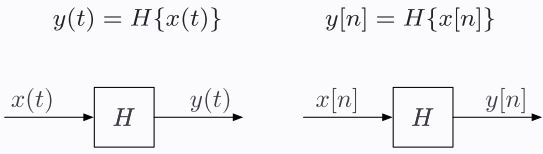
\includegraphics[scale=0.5]{Ex1.JPG}
  \end{figure}
  \item Two important types of operations $H$:
  \begin{itemize}
    \item Linear or non-linear function
    \item Time-invariant or time-varying function
  \end{itemize}
\end{itemize}

\pagebreak
%%%%%%%%%%%%%%%%%%%%%%%%%%%%%%%%%%%%%%%%%%%%%%%%%%%%%%%%%%%%%%%%%%%%%%%%%%%%%%%%%%%%%%%%%%%%%%%%%%%%%%%%%%
\subsection{Properties of a LTI system}

\begin{itemize}
  \item Linearity: Satisfies \textbf{superposition} and \textbf{homogeneity}
  \begin{align*}
    x(t) &= \sum_{i=1}^N a_i x_i(t) \\
    y(t) &= \sum_{i=1}^N a_i y_i(t) 
  \end{align*}
  \begin{itemize}
    \item Superposition: 
    \begin{itemize}
      \item Input: $x_1(t)$ and $x_2(t)$
      \item Output: $y_1(t)$ and $y_2(t)$
    \end{itemize}
    $$
      x_1(t) + x_2(t) = y_1(t) + y_2(t)
    $$

    \item Homogeneity:
    \begin{itemize}
      \item Input: $x_1(t)$ 
      \item Output: $y_1(t)$
    \end{itemize}
    \begin{align*}
      x_1(t) &= y_1(t) \\
      a*x_1(t) &= a*y_1(t)
    \end{align*}
  \end{itemize}

  \item Time-invariance: $H$ does not change over time 
  \begin{itemize}
    \item Time-shift in input equals time-shift of output
  \end{itemize}

  \item Memory and memoryless systems: 
  \begin{itemize}
    \item \textbf{Memoryless}: Function depends on current input
    \item \textbf{Memory}: Function depends on past and future inputs
  \end{itemize}

  \item Stability: Stable if output bounded if input bounded 
  \item \textbf{BIBO}: Bounded-input, bounded-output
  \begin{align*}
    |y(t)| \leq M_y < \infty \; \text{given} \; |x(t)| \leq M_x < \infty
  \end{align*}
  where $M_x$ and $M_y$ are finite positive bounds 

  \item Most linear system applications require BIBO stability
  
  \item Causality: Output depends on \textbf{past} and \textbf{present} inputs
  $$
    y[n] = 0.25(x[n] + x[n - 1] + x[n - 2] + x[n - 3])
  $$

  \item \textbf{Non-causal}: Present, future and past input required
  $$
    y[n] = 0.25(x[n + 2] + x[n + 1] + x[n] + x[n - 1])
  $$

  \item \textbf{Anticausal}: Only future signal required 
  $$
    y[n] = 0.33(x[n + 3] + x[n + 2] + x[n + 1])
  $$
\end{itemize}










%%%%%%%%%%%%%%%%%%%%%%%%%%%%%%%%%%%%%%%%%%%%%%%%%%%%%%%%%%%%%%%%%%%%%%%%%%%%%%%%%%%%%%%%%%%%%%%%%%%%%%%%%%
\end{document}
